\chapter[Elasticidad]{ELASTICIDAD}
\startcontents
\printchaptertableofcontents

En las páginas que siguen, exploraremos un concepto central de la mecánica de sólidos: la \textbf{elasticidad}. Esta propiedad de los materiales es la base de numerosos campos de la ciencia y la ingeniería, permitiéndonos comprender y predecir cómo se comportan las estructuras bajo la acción de fuerzas externas. En este capítulo aprenderemos que es un cuerpo elástico, sus propiedades fundamentales y como se aplican los esfuerzos y deformaciones en situaciones de la vida cotidiana.

\section{Conceptos Fundamentales}

Para adentrarnos en este fascinante campo, es esencial comenzar por definir los conceptos básicos que rigen el comportamiento de los materiales bajo carga.

La \textbf{elasticidad} es la parte de la estática\footnote{La estática es la rama de la mecánica que estudia los cuerpos en equilibrio.} que estudia cómo se deforman los \textbf{cuerpos elásticos}\footnote{La definición se muestra en la página.} debido a la aplicación de fuerzas externas que se ejercen sobre ellos.

\begin{definition}{}{}
    Entendemos por \textbf{deformación} el cambio en las dimensiones y/o la forma de un cuerpo causado por la aplicación de fuerzas externas ejercidas sobre él.
\end{definition}

Un \textbf{cuerpo rígido ideal} sería aquel que no sufre deformación alguna al ejercer fuerzas sobre él.

Consideremos un cuerpo de material homogéneo\footnote{Un material homogéneo es aquel que tiene la misma densidad en todas partes.}, sobre el cual se han aplicado fuerzas externas que lo deformaron.

Si al suprimir las fuerzas deformadoras sobre él, éste recupera del todo su forma y dimensiones originales decimos que el material es \textbf{perfectamente elástico}. Si las recupera en un alto porcentaje diremos que el material es \textbf{elástico}. Si no las recupera en absoluto diremos que el material es \textbf{perfectamente plástico} y si las recupera en un pequeño porcentaje diremos que el material es \textbf{plástico} y que sufrió una \textbf{deformación plástica}.

En el mundo real todos los materiales presentan comportamientos elásticos y también plásticos dependiendo de la magnitud de las fuerzas deformadoras. Si la magnitud de las fuerzas deformadoras es muy pequeña es casi seguro que el comportamiento de la mayoría de los materiales es elástico; pero si las magnitudes de esas fuerzas son grandes entonces tendremos deformaciones plásticas hasta llegar a la ruptura del material. Los materiales elásticos almacenan energía mecánica al ser deformados, mientras que los materiales plásticos convierten la energía mecánica de la deformación en energía interna al incrementar su temperatura. Una aplicación muy importante del estudio de las propiedades mecánicas de los materiales, como son las propiedades elásticas, es la deformación progresiva de los materiales que rodean el habitáculo de los pasajeros en un automóvil, con la finalidad de proteger la integridad física de los mismos.

Para explicar el fenómeno de la deformación de los cuerpos elásticos usamos una cantidad física escalar denominada \textbf{esfuerzo}.
\begin{definition}{}{esfuerzo}
    El esfuerzo es el cociente de la magnitud de la fuerza deformadora entre el área de alguna sección del cuerpo deformado. Es decir,
    $$\text{Esfuerzo}=\frac{\text{Fuerza}}{\text{Área}}.$$
    Además, la unidad física del esfuerzo en el Sistema Internacional de Unidades es el \textbf{Pascal}:
    $$1\text{ Pascal} = \frac{1\text{ Newton}}{m^2}$$
\end{definition}

\section{Comportamiento del Material}

La mayoría de los elementos que integran una máquina como son los engranes, los ejes, las poleas, pernos, tornillos, remaches, baleros y otras piezas, son sometidos a esfuerzos longitudinales (\textbf{tensión} o \textbf{compresión}) o \textbf{transversales} (esfuerzo cortante) o en algunos casos menos frecuentes a \textbf{esfuerzos de presión hidrostática}. La mayoría de estos elementos mecánicos están hechos de metales como el acero, el aluminio o aleaciones. Cuando los esfuerzos a los que se someten los metales no son muy grandes, éstos se comportan de manera elástica. En la Figura \ref{fig:E_vs_Du} se muestra la gráfica del esfuerzo de tensión $E$ (expresado en Mega Pascales), al que se somete un alambre de acero, contra la deformación unitaria $Du$ (adimensional) que éste experimenta. El alambre de un metro de longitud y de un milímetro de diámetro, en posición vertical, está sujeto firmemente en su extremo superior a un soporte rígido. Se le van colgando pesas de diferente masa y a partir de los \SI{3.45}{\kilogram} se empieza a deformar de manera plástica. Esto significa que el comportamiento lineal (\textbf{comportamiento elástico}) entre esfuerzo y deformación unitaria dejo de cumplirse. El alambre ya no obedece la ley de Hooke porque se rebasó el \textbf{límite elástico} y a partir de ese momento comienza la deformación acelerada hasta llegar a la \textbf{ruptura} del alambre.
\begin{figure}
    \centering
    \begin{tikzpicture}[scale=0.85,font=\small]
        % --- Líneas de referencia ---
        \draw[red!0, name path=A--A'] (0,6) -- ++(6,0);
        \draw[red!0, name path=C--C'] (0,8) -- ++(11,0);
    
        % --- Definición de la curva y cálculo de intersecciones ---
        \path[name path=f--f'] (0,0) .. controls (1,3) and (3,8) .. (11,8);
        
        % --- Calculamos las intersecciones ---
        \path[name intersections={of=A--A' and f--f', by=B}];
        \path[name intersections={of=C--C' and f--f', by=D}];
    
        % --- Relleno curvo usando clip ---
        \begin{scope}
            \clip (0,0) rectangle (B);
            \fill[azul!20] (0,0) .. controls (1,3) and (3,8) .. (11,8) -- (0,6) -- cycle;
        \end{scope}
    
        \begin{scope}
            \clip (0,6) rectangle (13,8);
            \fill[verde!40,opacity=0.7] (0,0) .. controls (1,3) and (3,8) .. (11,8) -- (0,8) -- cycle;
        \end{scope}
    
        % --- Dibujo final de la curva sobre el relleno ---
        \draw[mainc,ultra thick] (0,0) .. controls (1,3) and (3,8) .. (D);
    
        \fill[Gold] (B) circle (0.7mm);
        \fill[rojo] (D) circle (0.7mm);
    
        \foreach \y in {0.5,1,...,8} {
            \draw[shift={(0,\y)},color=black] (0,0) -- (-1.1mm,0);
        }
        
        \foreach \x in {0.5,1,...,12} {
            \draw[shift={(\x,0)},color=black] (0,0) -- (0,-1.1mm);
        }
    
        % --- Ejes ---
        \draw[-stealth,very thick] (-0.5,0) -- ++(13,0) node[below] {$Du$ $(\times 10^{-4})$};
        \draw[-stealth,very thick] (0,-0.5) -- ++(0,9) node[above] {$E$ (MPa)};
    
        % --- Leyenda ---
        \matrix[
            draw=gray,
            line width=0.4mm,
            fill=white,
            right,
            at={($(current bounding box.center)+(0,1)$)},
            nodes={anchor=west,font=\footnotesize},
            inner sep=1mm,
            column sep=1mm,
            rounded corners,
            column 1/.style={nodes={anchor=center}}, % Centra el contenido de la columna 1
        ]
        {

            % --- Fila 1: Curva principal ---
            \draw[mainc,line width=0.36mm] (-0.2,0) -- (0.2,0); &
            \node {Curva de Esfuerzo}; \\
        
            % --- Fila 2: Punto de intersección ---
            \fill[Gold] (0,0) circle (0.6mm); &
            \node {Límite Elástico}; \\

            % --- Fila 3: Punto de intersección ---
            \fill[rojo] (0,0) circle (0.6mm); &
            \node {Ruptura del material}; \\
        };
    \end{tikzpicture}
    \caption{Gráfica del Esfuerzo $E$ contra la deformación unitaria $Du$.}
    \label{fig:E_vs_Du}
\end{figure}
Este comportamiento es típico de los metales, piense por ejemplo en los cables de acero que mueven la cabina de un ascensor, por seguridad los esfuerzos de tensión sobre ellos no pueden rebasar el límite elástico. A la gráfica anterior también se la conoce como \textbf{diagrama esfuerzo-deformación}.\\
Si aumentamos el esfuerzo más allá del límite elástico, el material entra en la etapa de deformación plástica y ya no recuperará su forma y dimensiones originales. Si estando en esta etapa de deformación dejamos que de manera gradual el material se relaje disminuyendo poco a poco el esfuerzo, veremos que la trayectoria que se sigue en el diagrama esfuerzo-deformación (\textbf{curva de relajación}) ya no será igual a la inicial (\textbf{curva de carga}), y finalmente al suprimir el esfuerzo el material quedará deformado (ver Figura \ref{fig:curva_relajacion}).
\begin{figure}
    \centering
    \begin{tikzpicture}[scale=0.85,font=\small]
        % --- Líneas de referencia ---
        \draw[red!0, name path=A--A'] (0,6) -- ++(6,0);
        \draw[red!0, name path=C--C'] (0,8) -- ++(11,0);
    
        % --- Definición de la curva de Esfuerzo ---
        \path[name path=f--f'] (0,0) .. controls (1,3) and (3,8) .. (11,8);
        
        % --- Calculamos las intersecciones ---
        \path[name intersections={of=A--A' and f--f', by=B}];
        \path[name intersections={of=C--C' and f--f', by=D}];
    
        % --- Definición de la curva de Relajación ---
        \path[name path=f2--f2'] (1.5,0) .. controls (3,5) and (4.35,8) .. (D);
    
        % --- Calculo de la intersección ---
        \path[name intersections={of=f--f' and f2--f2',by=E}];
        
        % --- Relleno curvo usando clip ---
        \begin{scope}
            \clip (0,0) rectangle (B);
            \fill[azul!20] (0,0) .. controls (1,3) and (3,8) .. (11,8) -- (0,6) -- cycle;
        \end{scope}
        
        \begin{scope}
            \clip (0,6) rectangle (13,8);
            \fill[verde!40,opacity=0.7] (0,0) .. controls (1,3) and (3,8) .. (11,8) -- (0,8) -- cycle;
        \end{scope}
    
        \begin{scope}
            \clip (0,0) .. controls (1,3) and (3,8) .. (11,8) -- (11,0) -- (0,0) -- cycle;
            \draw[curva vectorial=grisa] (E) .. controls (4,6) and (3,4) .. (1.5,0);
        \end{scope}
        
        % --- DIBUJO DE LAS CURVAS USANDO DECORATIONS ---
        % \draw[curva vectorial=grisa] (E) .. controls (4.35,8) and (3,5) .. (1.5,0);
        \draw[curva vectorial=mainc] (0,0) .. controls (1,3) and (3,8) .. (D);
        
        % --- Puntos de intersección ---
        \fill[Gold] (B) circle (0.7mm);
        \fill[rojo] (D) circle (0.7mm);
        
        \foreach \y in {0.5,1,...,8} {
            \draw[shift={(0,\y)},color=black] (0,0) -- (-1.1mm,0);
        }
        
        \foreach \x in {0.5,1,...,11.5} {
            \draw[shift={(\x,0)},color=black] (0,0) -- (0,-1.1mm);
        }
        
        % --- Ejes ---
        \draw[-stealth,very thick] (-0.5,0) -- ++(12.5,0) node[below] {$Du$ $(\times 10^{-4})$};
        \draw[-stealth,very thick] (0,-0.5) -- ++(0,9) node[above] {$E$ (MPa)};
        
        % --- Leyenda ---
        \matrix[
            draw=gray,
            line width=0.4mm,
            fill=white,
            right,
            at={($(current bounding box.center)+(2,0)$)},
            nodes={anchor=west,font=\footnotesize},
            inner sep=1mm,
            column sep=1mm,
            rounded corners,
            column 1/.style={nodes={anchor=center}}
        ]
        {
            % --- Fila 1: Curva principal ---
            \draw[vector,mainc,line width=0.36mm] (-0.2,0) -- (0.2,0); &
            \node {Curva de Esfuerzo}; \\
    
            % --- Fila 2: Curva secundaria ---
            \draw[vector,grisa,line width=0.36mm] (-0.2,0) -- (0.2,0); &
            \node {Curva de Relajación}; \\
        
            % --- Fila 3: Punto de intersección ---
            \fill[Gold] (0,0) circle (0.6mm); &
            \node {Límite Elástico}; \\
    
            % --- Fila 4: Punto de intersección ---
            \fill[rojo] (0,0) circle (0.6mm); &
            \node {Ruptura del material}; \\
        };
    \end{tikzpicture}
    \caption{Ilustración del comportamiento plástico de un material. Al superar el límite elástico, si el esfuerzo se retira, el material no regresa por la curva de carga original, sino que sigue la curva de relajación, lo que ocasiona una deformación permanente.}
    \label{fig:curva_relajacion}
\end{figure}
Si la etapa de comportamiento plástico, antes de llegar a la ruptura, es duradera, diremos que el material es \textbf{dúctil}. En caso contrario, si la ruptura se da poco después de rebasar el límite elástico diremos que el material es \textbf{frágil}. Existen materiales anómalos como el caucho vulcanizado en los que se pierde el comportamiento lineal llegando a superar sus dimensiones originales hasta por siete veces, sin embargo, la curva de relajación termina en el origen y por lo tanto ¡es un material elástico! a este comportamiento se le llama \textbf{histéresis elástica}.

\section{Esfuerzos longitudinales}

Ahora que hemos explorado el comportamiento general de los materiales, podemos clasificar los esfuerzos según cómo se aplican las fuerzas. Los más comunes son los \textbf{esfuerzos longitudinales} y los \textbf{transversales}, aunque también existe el \textbf{esfuerzo de presión hidrostática} cuando un cuerpo es sometido a la presión de un fluido.

\subsection{Esfuerzo de tensión}

Consideremos una barra recta de sección transversal rectangular uniforme\footnote{La sección transversal es la superficie que resulta de la intersección de un plano imaginario, perpendicular a la barra, con la barra misma. Cuando decimos que es uniforme significa que esta superficie es igual en toda la longitud de la barra.}, de longitud $L_0$, colocada sobre una mesa horizontal. A continuación, aplicamos un par de fuerzas externas $\F$, $-\F$ de igual magnitud, pero de sentido opuesto, en los extremos de la barra de manera que la estiran véase la Figura \ref{fig:esfuerzo_tension}
\begin{figure}
    \centering
    \subfloat[]{
        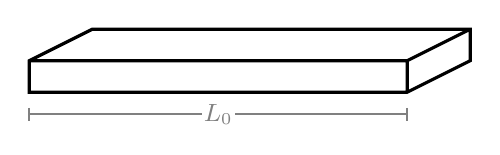
\begin{tikzpicture}[scale=0.8,font=\small]
            \fill[white] (0,0) -- ++(6,0) -- ++(1,0.5) -- ++(0,0.5) -- ++(-6,0) -- ++(-1,-0.5) -- cycle;
            \draw[line width=0.4mm] (0,0) -- ++(6,0) -- ++(1,0.5) -- ++(0,0.5) -- ++(-6,0) -- ++(-1,-0.5) -- cycle
                (0,0.5) -- ++(6,0) -- ++(1,0.5)
                (6,0) -- ++(0,0.5);
            \begin{scope}[gray,line width=0.25mm]
                \draw (0,-0.35) -- ++(6,0)  node[midway,fill=white,inner sep=0.8pt] {$L_0$};
                \foreach \x in {0,6} {
                    \draw[shift={(\x,-0.35)}] (0,1mm) -- (0,-1mm);
                }
            \end{scope}
        \end{tikzpicture}
    } \hfill
    \subfloat[]{
        \begin{tikzpicture}[scale=0.8,font=\small]
            \draw[vector,line width=0.4mm,azul](0.5,0.5) -- ++(-1.5,0) node[midway,above] {$-\F$};
            \fill[white] (0,0) -- ++(6,0) -- ++(1,0.5) -- ++(0,0.5) -- ++(-6,0) -- ++(-1,-0.5) -- cycle;
            \draw[line width=0.4mm] (0,0) -- ++(6,0) -- ++(1,0.5) -- ++(0,0.5) -- ++(-6,0) -- ++(-1,-0.5) -- cycle
                (0,0.5) -- ++(6,0) -- ++(1,0.5)
                (6,0) -- ++(0,0.5);
            \begin{scope}[gray,line width=0.25mm]
                \draw (0,-0.35) -- ++(6,0)  node[midway,fill=white,inner sep=0.7pt] {$L=L_0 + \DeltaL$};
                \foreach \x in {0,6} {
                    \draw[shift={(\x,-0.35)}] (0,1mm) -- (0,-1mm);
                }
            \end{scope}
            \draw[vector,line width=0.4mm,azul] (6.5,0.5) -- ++(1.5,0) node[midway,above] {$\F$};
        \end{tikzpicture}
    }
    \caption{}
    \label{fig:esfuerzo_tension}
\end{figure}

De este modo, la barra de sección rectangular qué reposa sobre la mesa se mantiene en equilibrio pues la suma de las fuerzas externas es igual a cero. Cómo resultado de la aplicación del par de fuerzas deformadoras en los extremos de la barra, tenemos un incremento $\DeltaL$ en su longitud original $L_0$.
\begin{definition}{}{deformacion}
    Llamamos \textbf{deformación} al incremento de la longitud, expresado por
    $$\DeltaL = L - L_0.$$
\end{definition}
\begin{definition}{}{deformacion_unitaria}
    Denominamos \textbf{deformación unitaria} o \textbf{deformación relativa} al cociente
    $$D_U = \frac{\DeltaL}{L_0}.$$
\end{definition}

Para este caso definimos el esfuerzo de tensión como
$$E_T = \frac{F}{A}$$
donde $F$ es la magnitud común de las fuerzas que producen la tensión de la barra y A es el área de la sección transversal uniforme de la barra.

Experimentalmente se verifica que existe una correlación lineal entre el esfuerzo de tensión y la deformación unitaria. Es decir
$$E_T = Y\,\frac{\DeltaL}{L_0}$$
donde la constante de proporcionalidad $Y$ conocida como \textbf{Módulo de Young} es una característica del material, la cual también llamaremos \textbf{constante elástica}.

Si bien hemos considerado una barra de sección transversal rectangular, el mismo resultado se obtiene para cualquier otro tipo de sección transversal: circular, cuadrada, hexagonal, etc.

En la siguiente tabla se muestran algunos valores del Módulo de Young en Pascales.

\begin{table}
    \centering
    \begin{NiceTabular}{cc}[hvlines-except-borders, cell-space-limits=4pt, rules={color=white,width=1pt}]
        \CodeBefore
        \rowcolor{mainc!80}{1}
        \rowcolors{2}{mainc!30!white}{mainc!15!white}
        \Body
        \RowStyle[color=white]{}
        \RowStyle{\ipn\selectfont\bfseries}Material & \makecell{Módulo de Young \\ $\left(\SI{1e10}{\pascal}\right)$} \\
        Aluminio &  7.0 \\
        Latón    &  9.0 \\
        Cobre    & 11.0 \\
        Hierro   & 21.0 \\
        Plomo    &  1.6 \\
        Níquel   & 21.0 \\
        Acero    & 20.0
    \end{NiceTabular}
    \caption{Módulo de Young de algunos materiales.}
    \label{tab:Modulo_Young}
\end{table}

El \textbf{Módulo de Young} no solo cuantifica la resistencia de un material a ser estirado, sino también su resistencia a ser acortado. De manera análoga al esfuerzo de tensión, podemos analizar el caso opuesto, donde las fuerzas externas actúan para comprimir el objeto en lugar de alargarlo.

% \begin{semblanza}{Thomas Young}{1773-1829}[Young.jpg]
%     Thomas Young (1773-1829) fue un prodigio de la Inglaterra de la Regencia, una mente tan vasta y versátil que su figura roza lo legendario. Nacido en una familia cuáquera que fomentó su precoz intelecto —se dice que leía con fluidez a los dos años—, Young se formó como médico en las universidades más prestigiosas de Europa. Sin embargo, su práctica médica, aunque respetable, fue solo el telón de fondo para una deslumbrante carrera científica que llevó a cabo en gran medida por pura pasión intelectual, consolidándolo como el polímata por excelencia.

%     La contribución que inmortalizó a Young fue su audaz desafío a la autoridad de Isaac Newton. Durante más de un siglo, la física había aceptado que la luz estaba compuesta por partículas (corpúsculos). Young, a través de su \textbf{experimento de la doble rendija} (circa 1801), ofreció una prueba elegante e irrefutable de lo contrario. Al hacer pasar un haz de luz a través de dos finas rendijas paralelas, observó que en la pantalla de fondo no aparecían dos simples líneas de luz, sino un patrón de bandas brillantes y oscuras alternadas. Este fenómeno, conocido como \textbf{interferencia}, solo podía explicarse si la luz se comportaba como una onda, donde las crestas de diferentes ondas se suman (interferencia constructiva, creando luz) o se anulan (interferencia destructiva, creando oscuridad). Este resultado no solo resucitó la teoría ondulatoria, sino que se convirtió en una piedra angular de la física, presagiando las dualidades de la mecánica cuántica.
    
%     Pero el genio de Young no conocía fronteras. Como médico, fue el primero en describir el \textbf{astigmatismo} y sus estudios sobre la percepción del color culminaron en la \textbf{teoría tricromática de Young-Helmholtz}, que postula que nuestra visión del color es el resultado de la activación de tres tipos de fotorreceptores en la retina, sensibles al rojo, verde y azul. Su mente analítica también descifró enigmas de la antigüedad; en el campo de la egiptología, fue el primero en deducir que los cartuchos de la \textbf{Piedra de Rosetta} contenían nombres fonéticos de los faraones, como ``Ptolomeo''. Este fue el avance conceptual clave que permitió a Jean-François Champollion descifrar por completo los jeroglíficos. Desde la elasticidad de los materiales con su famoso \textbf{Módulo de Young} hasta la teoría de las mareas, Thomas Young demostró ser un gigante intelectual cuyo legado une la física, la fisiología y la historia.
% \end{semblanza}

\subsection{Esfuerzo de compresión}

Considerando la misma barra del caso anterior con la diferencia de que ahora las fuerzas externas tienen sentidos contrarios, de modo que comprimen la barra (ver Figura \ref{fig:esfuerzo_compresion}).

\begin{figure}
    \centering
    \subfloat[]{
        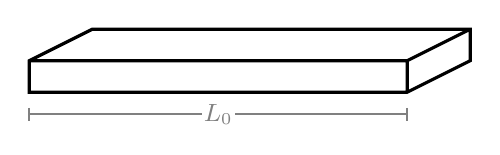
\begin{tikzpicture}[scale=0.8,font=\small]
            \fill[white] (0,0) -- ++(6,0) -- ++(1,0.5) -- ++(0,0.5) -- ++(-6,0) -- ++(-1,-0.5) -- cycle;
            \draw[line width=0.4mm] (0,0) -- ++(6,0) -- ++(1,0.5) -- ++(0,0.5) -- ++(-6,0) -- ++(-1,-0.5) -- cycle
                (0,0.5) -- ++(6,0) -- ++(1,0.5)
                (6,0) -- ++(0,0.5);
            \begin{scope}[gray,line width=0.25mm]
                \draw (0,-0.35) -- ++(6,0)  node[midway,fill=white,inner sep=0.8pt] {$L_0$};
                \foreach \x in {0,6} {
                    \draw[shift={(\x,-0.35)}] (0,1mm) -- (0,-1mm);
                }
            \end{scope}
        \end{tikzpicture}
    } \hfill
    \subfloat[]{
        \begin{tikzpicture}[scale=0.8,font=\small]
            \draw[vector,line width=0.4mm,azul](-1,0.5) -- ++(1.5,0) node[midway,above] {$-\F$};
            \fill[white] (0,0) -- ++(6,0) -- ++(1,0.5) -- ++(0,0.5) -- ++(-6,0) -- ++(-1,-0.5) -- cycle;
            \draw[line width=0.4mm] (0,0) -- ++(6,0) -- ++(1,0.5) -- ++(0,0.5) -- ++(-6,0) -- ++(-1,-0.5) -- cycle
                (0,0.5) -- ++(6,0) -- ++(1,0.5)
                (6,0) -- ++(0,0.5);
            \begin{scope}[gray,line width=0.25mm]
                \draw (0,-0.35) -- ++(6,0)  node[midway,fill=white,inner sep=0.7pt] {$L=L_0 + \DeltaL$};
                \foreach \x in {0,6} {
                    \draw[shift={(\x,-0.35)}] (0,1mm) -- (0,-1mm);
                }
            \end{scope}
            \draw[vector,line width=0.4mm,azul] (8,0.5) -- ++(-1.5,0) node[midway,above] {$\F$};
        \end{tikzpicture}
    }
    \caption{}
    \label{fig:esfuerzo_compresion}
\end{figure}

En este caso la deformación $\DeltaL$ es negativa pues $L < L_0$ y el \textbf{esfuerzo de compresión}
$$E_C = \frac{F}{A}$$
que es una cantidad positiva, es directamente proporcional al valor absoluto de la deformación unitaria. Es decir
$$E_C = -Y\,\frac{\DeltaL}{L_0}$$
donde la constante de proporcionalidad sigue siendo el Módulo de Young. Para la mayoría de los materiales el Módulo de Young del esfuerzo de tensión es igual al del esfuerzo de compresión. En el caso de los huesos esto no se cumple.
A los esfuerzos de tensión y compresión se les conoce como también como esfuerzos longitudinales, ya que el esfuerzo (fuerza/área) se mantiene a lo largo de cualquier sección transversal de la barra.

Mientras que los esfuerzos longitudinales estiran o comprimen un material, existe otro tipo de esfuerzo que no busca cambiar la longitud del objeto, sino deformar su forma deslizando unas capas del material sobre otras. Este fenómeno, conocido como \textbf{esfuerzo transversal}, el cual es fundamental para entender la torsión y el cizallamiento en estructuras.

\section{Esfuerzo transversal}

Por simplicidad, consideremos ahora un bloque rectangular al cual se le han soldado dos placas: Una en la cara superior y otra en la inferior como se muestra en la figura (a). El bloque descansa firmemente sobre una mesa lisa y horizontal. A continuación, aplicamos sobre las placas un par de fuerzas externas horizontales $F\,$ y $-F\,$ de igual magnitud, pero opuestas en dirección, de manera que se alejan entre sí, ver figura (b). Como consecuencia de la aplicación de estas fuerzas, el bloque sufre una inclinación (deformación) que puede medirse por el ángulo $\phi$, en radianes, respecto a la vertical, o bien por la tangente del ángulo ya que el ángulo es muy pequeño si estamos dentro del comportamiento elástico del material. A diferencia de los esfuerzos longitudinales de tensión y compresión, en donde las fuerzas externas producen pares de fuerzas $F\,$ y $-F\,$ \textbf{perpendiculares} a cualquier sección transversal $A$ en todo lo largo de la barra; en el \textbf{esfuerzo cortante} se producen pares de fuerzas $F\,$ y $-F\,$ \textbf{paralelas} a cualquier sección transversal $A$ en todo lo alto del bloque.
\begin{figure}
    \centering
    \subfloat[]{
        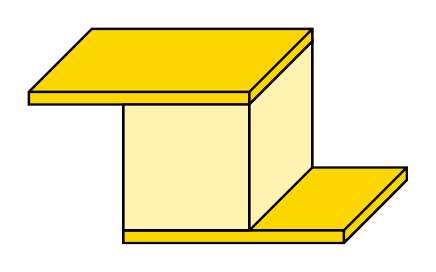
\begin{tikzpicture}[scale=0.8, line width=0.3mm]
            \filldraw[fill=Gold] (0,0) -- ++(0,-0.2) -- ++ (3.5,0) -- ++(1,1) -- ++(0,0.2) -- ++(-3.5,0) -- cycle
                (0,0) -- ++(3.5,0) -- ++(1,1)
                (3.5,0) -- ++(0,-0.2);
        
            \filldraw[fill=Gold] (-1.5,2.2) -- ++(0,-0.2) -- ++(3.5,0) -- ++(1,1) -- ++(0,0.2) -- ++(-3.5,0) -- cycle
                (-1.5,2.2) -- ++(3.5,0) -- ++(1,1)
                (2,2.2) -- ++(0,-0.2);
        
            \filldraw[fill=Gold!30] (0,0) -- ++(2,0) -- ++(1,1) -- ++(0,2) -- ++(-1,-1) -- ++(-2,0) -- cycle
                (2,2) -- ++(0,-2);
        \end{tikzpicture}
    } \hfill
    \subfloat[]{
        \begin{tikzpicture}[scale=0.8,font=\scriptsize, line width=0.3mm]
            \coordinate (O) at (3.5,1);
            \coordinate (A) at (2.5,3);
            \coordinate (B) at (3.5,3);
            
            \draw[vector,azul,line width=0.6mm] (-1.5,2.6) -- ++(-1,0) node[left] {$-F$};
            
            \filldraw[fill=Gold] (0.5,0) -- ++(0,-0.2) -- ++ (3.5,0) -- ++(1,1) -- ++(0,0.2) -- ++(-3.5,0) -- cycle
                (0.5,0) -- ++(3.5,0) -- ++(1,1)
                (4,0) -- ++(0,-0.2);
        
            \filldraw[fill=Gold] (-2,2.2) -- ++(0,-0.2) -- ++(3.5,0) -- ++(1,1) -- ++(0,0.2) -- ++(-3.5,0) -- cycle
                (-2,2.2) -- ++(3.5,0) -- ++(1,1)
                (1.5,2.2) -- ++(0,-0.2);
        
            \filldraw[fill=Gold!30] (0.5,0) -- ++(2,0) -- ++(1,1) -- ++(-1,2) -- ++(-1,-1) -- ++(-2,0) -- cycle
                (1.5,2) -- ++(1,-2);
        
            \draw[vector,azul,line width=0.6mm] (4.5,0.4) -- ++(1,0) node[right] {$F$};
        
            \draw[dash pattern=on 1.5mm, gray] (0,1) node[left] {$A$} -- ++(2,0) -- ++(1,1);
        
            \draw[azul] (O) -- (B) node[midway,right] {$h$};
        
            \pic [draw=rojo,angle radius=8mm,angle eccentricity=1.25,"\textcolor{rojo}{$\phi$}"] {angle=B--O--A};
        
            \draw[latex-latex,verde] (A) -- (B) node[midway,above] {$\Deltax$};
        \end{tikzpicture}
    }
    \caption{Caption}
    \label{fig:}
\end{figure}
\begin{definition}{}{}
    Definimos el \textbf{esfuerzo cortante} o \textbf{esfuerzo de cizalla} como
    $$E_Z = \frac{F}{A}.$$
    Además, la deformación unitaria, en este caso, una cantidad adimensional, es la tangente del ángulo de inclinación
    $$D_U = \frac{\Deltax}{h} = \tan{\phi} \cong \phi$$
\end{definition}
La relación de proporcionalidad directa entre el esfuerzo cortante y la deformación unitaria causada, la cual se verifica experimentalmente, es
$$\frac{F}{A} = \mu\phi$$
donde la constante de proporcionalidad $\mu$ llamada \textbf{módulo de rigidez} es una característica del material.

En la siguiente tabla se muestran algunos valores del módulo de rigidez en Pascales.
\begin{table}
    \centering
    \begin{NiceTabular}{cc}[hvlines-except-borders, cell-space-limits=4pt, rules={color=white,width=1pt}]
        \CodeBefore
        \rowcolor{mainc!80}{1}
        \rowcolors{2}{mainc!30!white}{mainc!15!white}
        \Body
        \RowStyle[color=white]{}
        \RowStyle{\ipn\selectfont\bfseries}Material & \makecell{Módulo de rigidez $\mu$ \\ $\left(\SI{1e10}{\pascal}\right)$} \\
        Aluminio & 2.5 \\
        Latón    & 3.5 \\
        Cobre    & 4.4 \\
        Hierro   & 7.7 \\
        Plomo    & 0.6 \\
        Níquel   & 7.8 \\
        Acero    & 7.5
    \end{NiceTabular}
    \caption{Módulo de Young de algunos materiales.}
    \label{tab:my_label_2}
\end{table}

Ya hemos analizado cómo responden los sólidos a fuerzas aplicadas en una sola dirección, ya sean perpendiculares (tensión/compresión) o paralelas (cortante) a una superficie. Ahora, consideremos un caso más general: ¿qué sucede cuando un cuerpo es sometido a fuerzas uniformes en \textit{todas} sus caras simultáneamente, como ocurre al sumergirlo en un fluido a presión? Este escenario nos introduce al concepto de esfuerzo volumétrico.

\section{Esfuerzo de presión hidrostática}

El \textbf{esfuerzo de presión hidrostática} es igual al incremento de la presión que ejerce un líquido sobre la superficie de un cuerpo sumergido en él. En la figura se muestra un recipiente cilíndrico provisto de un émbolo que cubre la superficie del líquido dentro de él, en el cual se encuentra sumergido un objeto, en nuestro caso un bloque. Dado que los líquidos son prácticamente incompresibles al aplicar una fuerza $F$ sobre el émbolo de área $A$ se produce un incremento $\Deltap$ en la presión de cada punto del interior del líquido (principio de Pascal).
$$\Deltap = \frac{F}{A}.$$
Este esfuerzo es proporcional a la deformación unitaria que experimenta el volumen inicial $V_0$ del cuerpo
$$D_U = \frac{\DeltaV}{V_0}$$
Dado que un incremento positivo de la presión hidrostática produce una reducción del volumen del cuerpo sumergido, la deformación unitaria es negativa, por lo tanto, la relación de proporcionalidad directa entre el esfuerzo de presión hidrostática y la deformación unitaria del volumen se escribe como
$$\Deltap = \frac{F}{A} = -B\frac{F}{A}$$
donde $B$ es el \textbf{módulo de compresibilidad volumétrico} que es una característica del material sumergido.

El inverso del módulo de compresibilidad volumétrico se llama \textbf{coeficiente de compresibilidad}
% \sideFigure[\label{fig:presion-hidrostatica}]{
%     \begin{tikzpicture}[scale=0.5, transform shape, line width=0.45mm]
%         \fill[Snow3] (-3,0) arc (180:360:3cm and 1cm) -- ++(0,7) arc (0:180:3cm and 1cm) -- cycle;
%         \fill[SteelBlue1!80] (-3,0) arc (180:0:3cm and 1cm)-- ++(0,5.3) arc (360:180:3cm and 1cm) -- cycle;
%         \fill[SteelBlue1!80] (0,0) ellipse (3cm and 1cm); 
%         \filldraw[fill=brown] (0,6.3) ellipse (3cm and 1cm);
%         \draw[fill=brown] (-3,6.3) -- ++(0,-1) arc (180:360:3cm and 1cm) -- ++(0,1) arc (360:180:3cm and 1cm);
%         \draw[fill=brown] (0,7) ellipse (1cm and 0.33cm);
%         \draw (-1,7) -- ++(0,-0.5) arc (180:360:1cm and 0.33cm) -- ++(0,0.5);
%         \begin{scope}
%             \path[fill=Snow3, draw=black, even odd rule] (-3.1,0) arc(180:0:3.1cm and 1.1cm) -- ++(-0.1,0) arc(0:180:3cm and 1cm);
%             \path[fill=Snow3, draw=black, even odd rule] (-3.1,7) -- ++(0,-7) arc(180:360:3.1cm and 1.1cm) -- ++(0,7) -- ++(-0.1,0) -- ++(0,-7) arc(360:180:3cm and 1cm) -- ++(0,7) -- cycle;
%             \path[fill=Snow3, even odd rule, draw=black]
%                 (0,7) ellipse [x radius=3.1cm, y radius=1.1cm]
%                 (0,7) ellipse [x radius=3cm, y radius=1cm];
%         \end{scope}
%         \begin{scope}[vector,line width=1mm,rojo]
%             \draw (-2,1) -- ++(1,0);
%             \draw (0,-1) -- ++(0,1);
%         \end{scope}
%         \draw[fill=azul!80] (-1.25,-0.25) -- ++(2,0) -- ++(0.5,0.5) -- ++(0,2) -- ++(-2,0) -- ++(-0.5,-0.5) -- cycle
%             (-1.25,1.75) -- ++(2,0) -- ++(0.5,0.5)
%             (0.75,-0.25) -- +(0,2);
%         \begin{scope}[vector,line width=1mm,rojo]
%             \draw (0,9) node[anchor=north west] {$F$} -- ++(0,-2);
%             \draw (0,3) node[above] {$p$} -- ++(0,-1);
%             \draw (2,1) -- ++(-1,0);
%             \draw (-0.95,0.25) -- ++(0.7,0.5);
%         \end{scope}
%     \end{tikzpicture}
% }
$$k = \frac{1}{B} = \frac{\DeltaV}{\Deltap V_0}.$$
\begin{figure}
    \centering
    \begin{tikzpicture}[line width=0.45mm]
        % ====== Recipiente (parte exterior en gris claro) ======
        % Cuerpo del contenedor (elipse inferior + paredes + elipse superior)
        \fill[Snow3] (-3,0) arc (180:360:3cm and 1cm) -- ++(0,7) arc (0:180:3cm and 1cm) -- cycle;
    
        % ====== Líquido (en azul) ======
        % Masa de líquido dentro del contenedor (elipse inferior + paredes + nivel superior)
        \fill[SteelBlue1!80] (-3,0) arc (180:0:3cm and 1cm)-- ++(0,5.3) arc (360:180:3cm and 1cm) -- cycle;
    
        % Superficie del líquido (elipse azul en la base)
        \fill[SteelBlue1!80] (0,0) ellipse (3cm and 1cm);
        
        % ====== Tapa y parte superior (en marrón) ======
        % Base sólida de la tapa superior
        \filldraw[fill=brown] (0,6.3) ellipse (3cm and 1cm);
        
        % Parte lateral de la tapa (pared cilíndrica marrón)
        \draw[fill=brown] (-3,6.3) -- ++(0,-1) arc (180:360:3cm and 1cm) -- ++(0,1) arc (360:180:3cm and 1cm);
    
        % Tapón superior (elipse pequeña marrón)
        \draw[fill=brown] (0,7) ellipse (1cm and 0.33cm);
    
        % Pared lateral del tapón
        \draw (-1,7) -- ++(0,-0.5) arc (180:360:1cm and 0.33cm) -- ++(0,0.5);
    
        % ====== Borde y contorno exterior ======
        \begin{scope}
            % Elipse inferior doble (contorno externo)
            \path[fill=Snow3, draw=black, even odd rule] 
                (-3.1,0) arc(180:0:3.1cm and 1.1cm) -- ++(-0.1,0) arc(0:180:3cm and 1cm);
            
            % Pared lateral doble del contenedor
            \path[fill=Snow3, draw=black, even odd rule] 
                (-3.1,7) -- ++(0,-7) arc(180:360:3.1cm and 1.1cm) -- ++(0,7) 
                -- ++(-0.1,0) -- ++(0,-7) arc(360:180:3cm and 1cm) -- ++(0,7) -- cycle;
            
            % Elipse superior doble (contorno de la boca del recipiente)
            \path[fill=Snow3, even odd rule, draw=black]
                (0,7) ellipse [x radius=3.1cm, y radius=1.1cm]
                (0,7) ellipse [x radius=3cm, y radius=1cm];
        \end{scope}
    
        % ====== Vectores internos (flechas rojas dentro del líquido) ======
        \begin{scope}[vector,line width=1mm,rojo]
            \draw (-2,1) -- ++(1,0);   % flecha horizontal
            \draw (0,-1) -- ++(0,1);   % flecha vertical
        \end{scope}
    
        % ====== Objeto azul dentro del líquido ======
        \draw[fill=azul!80] 
            (-1.25,-0.25) -- ++(2,0) -- ++(0.5,0.5) -- ++(0,2) 
            -- ++(-2,0) -- ++(-0.5,-0.5) -- cycle
            % Parte superior del objeto azul
            (-1.25,1.75) -- ++(2,0) -- ++(0.5,0.5)
            % Unión lateral
            (0.75,-0.25) -- +(0,2);
    
        % ====== Vectores externos (flechas rojas con etiquetas) ======
        \begin{scope}[vector,line width=1mm,rojo]
            \draw (0,9) node[anchor=north west] {$F$} -- ++(0,-2);  % fuerza F
            \draw (0,3) node[above] {$p$} -- ++(0,-1);              % presión p
            \draw (2,1) -- ++(-1,0);                                % vector lateral
            \draw (-0.95,0.25) -- ++(0.7,0.5);                      % vector inclinado
        \end{scope}
    \end{tikzpicture}
    \caption{Caption}
    \label{fig:presion-hidrostatica}
\end{figure}
En la siguiente tabla se muestran algunos valores del módulo de compresibilidad volumétrico en Pascales.
\begin{table}
    \centering
    \begin{NiceTabular}{cc}[hvlines-except-borders, cell-space-limits=4pt, rules={color=white,width=1pt}]
        \CodeBefore
        \rowcolor{mainc!80}{1}
        \rowcolors{2}{mainc!30!white}{mainc!15!white}
        \Body
        \RowStyle[color=white]{}
        \RowStyle{\ipn\selectfont\bfseries}Material & \makecell{Módulo de compresibilidad \\ volumétrico $B$ $\left(\SI{1e10}{\pascal}\right)$} \\
        Aluminio &  7.5 \\
        Latón    &  6.0 \\
        Cobre    & 14.0 \\
        Hierro   & 16.0 \\
        Plomo    &  4.1 \\
        Níquel   & 17.0 \\
        Acero    & 16.0
    \end{NiceTabular}
    \caption{Módulo de Young de algunos materiales.}
    \label{tab:my_label_3}
\end{table}

Hemos visto que, dentro del límite elástico, todos los tipos de esfuerzo (longitudinal, cortante y volumétrico) guardan una relación de proporcionalidad directa con la deformación que producen. Esta observación fundamental se puede generalizar en una de las leyes más importantes de la mecánica de sólidos.

\section{Relaciones esfuerzo-deformación}

El principio fundamental que gobierna la relación lineal entre el esfuerzo y la deformación en la zona elástica es conocido como la \textbf{Ley de Hooke}. Para presentar esta ley, comenzaremos con su aplicación más clásica: la deformación de un resorte.

\subsection{Ley de Hooke}

La \textbf{ley de Hooke}, como comúnmente se le conoce en los libros de texto de física, hace referencia a la relación de proporcionalidad directa entre la \textbf{fuerza externa} que deforma a un resorte, ya sea estirándolo o comprimiéndolo, y la deformación $x$ que sufre el resorte
$$F_{\ext} = kx$$
o bien, a la \textbf{fuerza de restitución} o \textbf{resistencia} (la fuerza de reacción a la fuerza externa) que opone el resorte a la deformación
$$F_{\res} = -kx$$
donde la deformación se mide desde la posición del extremo libre relajado (cuando no hay fuerza) del resorte; el otro extremo del resorte está fijo a la pared (ver figura). A la constante de proporcionalidad $k$ se le llama \textbf{constante elástica del resorte}.
\begin{figure}
    \centering
    \begin{tikzpicture}% [scale=1.2]
        % === Parámetros ===
        \def\yTop{1.5}          % Altura del resorte en equilibrio
        \def\yBot{-1.5}         % Altura del resorte estirado
        \def\springTopLen{3.02} % Longitud efectiva del resorte arriba
        \def\springBotLen{5.02} % Longitud efectiva del resorte abajo
        \def\coilAmp{4mm}       % Amplitud de los resortes
        \def\coilSegTop{3mm}    % Segment length arriba
        \def\coilSegBot{5mm}    % Segment length abajo
        \def\massRadius{3.5mm}  % Radio de las masas
    
        % === Líneas de referencia ===
        \draw[dash pattern=on 1.5mm off 2mm,gray,line width=0.2mm] (4.2,2.5) -- ++(0,-4);
        \draw[dash pattern=on 1.5mm off 2mm,gray,line width=0.2mm] (6.2,-0.3) -- ++(0,-1.2);
        
        % === Pared y resorte en equilibrio (arriba) ===
        \fill[pattern=north west lines, pattern color=gray!80] (-0.3,0.5) rectangle (0,2.5);
        \begin{scope}[line width=0.35mm]
            \draw (0,0.5) -- (0,2.5);
            \draw (0,\yTop) -- ++(0.6,0);
            \draw[decorate,decoration={coil,amplitude=\coilAmp,segment length=\coilSegTop}] 
                (0.58,\yTop) -- ++(\springTopLen,0);
            \draw (\springTopLen+0.58,\yTop) -- ++(0.6,0);
        \end{scope}
    
        % === Pared y resorte estirado (abajo) ===
        \fill[pattern=north west lines, pattern color=gray!80] (-0.3,-2.5) rectangle (0,-0.5);
        \begin{scope}[line width=0.35mm]
            \draw (0,-2.5) -- (0,-0.5);
            \draw (0,\yBot) -- ++(0.6,0);
            \draw[decorate,decoration={coil,amplitude=\coilAmp,segment length=\coilSegBot}] 
                (0.58,\yBot) -- ++(\springBotLen,0);
            \draw (\springBotLen+0.58,\yBot) -- ++(0.6,0);
        \end{scope}
    
        % === Vectores de fuerza ===
        \begin{scope}[vector,line width=0.6mm,azul]
            \draw[rojo] (6.2,\yBot) -- ++(-2,0) node[midway,below] {$F_{\res}$};
            \draw (6.2,\yBot) -- ++(2,0) node[midway,below] {$F_{\ext}$};
            \draw (0,\yBot) -- ++(-2,0) node[midway,below] {$-F_{\ext}$};
        \end{scope}
    
        % === Etiquetas ===
        \begin{scope}[line width=0.1mm]
            \node[above] at (4.2,2.5) {$x=0$};
            \draw[stealth-stealth] (4.2,-0.5) -- ++(2,0) 
                node[midway,fill=white,inner sep=0.3mm] {$x$};
        \end{scope}
        
        % === Masas ===
        \shade[ball color=mainc] (4.2,\yTop) circle (\massRadius);
        \shade[ball color=mainc] (6.2,\yBot) circle (\massRadius);
    \end{tikzpicture}
    \caption{Representación de un resorte en su estado de equilibrio ($x=0$, arriba) y al ser estirado una distancia $x$ por una fuerza externa $F_{\ext}$ (abajo). La fuerza de restitución del resorte, $F_{\res}$, se opone a la deformación.}
    \label{fig:ley-de-hooke}
\end{figure}
A la relación de proporcionalidad directa entre el esfuerzo de tensión o compresión y la deformación unitaria
$$E_T = \frac{F}{A} = Y\,\frac{\DeltaL}{L_0} \qquad \text{o} \qquad E_C = \frac{F}{A} = -Y\,\frac{\DeltaL}{L_0}$$
también se le conoce como ley de Hooke. Si despejemos a la fuerza F deformadora en ambas expresiones tenemos
$$F = \left(\frac{YA}{L_0}\right)\DeltaL \qquad \text{o} \qquad \left(\frac{YA}{L_0}\right)(-\DeltaL)$$
Que son expresiones similares a la ley de Hooke donde $F$ es la fuerza externa, $\DeltaL$ es la deformación y
$$k = \frac{YA}{L_0}$$
es la “constante elástica” tipo resorte. Aquí estamos suponiendo que el área de la sección transversal no cambia al ser deformada la barra. Sabemos que un resorte estirado o comprimido almacena una energía mecánica potencial
$$U = \frac{1}{2}kx^2.$$
Por lo tanto, una barra sometida a esfuerzo de tensión o compresión también almacenará una energía mecánica potencial
$$U = \frac{1}{2}\left(\frac{YA}{L_0}\right)(\DeltaL)^2$$
O bien en función de la fuerza deformadora
$$U = \frac{1}{2}F(\DeltaL)$$
En otras palabras, ésta es la cantidad de energía que se requiere para deformar una barra al aplicar un esfuerzo de tipo longitudinal (tensión o compresión).

La Ley de Hooke, aplicada a sólidos, describe perfectamente la deformación en la misma dirección de la fuerza aplicada (el estiramiento $\Delta L$). Sin embargo, la deformación de un material rara vez ocurre en una sola dimensión. Intuitivamente, si estiramos una liga, notamos que no solo se alarga, sino que también se vuelve más delgada. El \textbf{Coeficiente de Poisson} es la medida que cuantifica este efecto secundario en las dimensiones transversales.

\subsection{Coeficiente de Poisson}

Cuando una barra rectangular se somete a un esfuerzo de tensión, causado por un par de fuerzas externas, la longitud de la barra aumenta una cantidad $\DeltaL$; pero sus dimensiones transversales disminuyen en las cantidades $\Deltah$ y $\Deltaom$ (ver figura).
\begin{figure}
    \centering
    \tdplotsetmaincoords{80}{12}
    \begin{tikzpicture}[line width=0.4mm, tdplot_main_coords]
        % --- COTA DE LONGITUD FINAL (L) ---
        % Dibuja las dos pequeñas líneas verticales y discontinuas que sirven de guía para la cota.
        \draw[gray,dash pattern=on 1mm, line width=0.2mm] (4.5,-1,-1) -- ++(0,0,-1.5)
              (-4.5,-1,-1) -- ++(0,0,-1.5);
        % Dibuja la línea horizontal principal de la cota y le añade el texto L = L0 + ΔL en el medio.
        % El "fill=white" crea un fondo blanco para que el texto sea legible.
        \draw[gray] (-4.5,-1,-2.5) -- ++(9,0,0) node[midway, fill=white, inner sep=0.7mm] {$L = L_0+\Delta L$};
        
        % --- COTA DE LONGITUD INICIAL (L0) ---
        % Dibuja la línea y la etiqueta para la longitud inicial (L0) por encima de la figura.
        \draw[gray] (-3,2.5,2) -- ++(6,0,0) node[midway, fill=white, inner sep=0.7mm] {$L_0$};
        
        % --- VECTOR DE FUERZA IZQUIERDO (-F) ---
        % Dibuja una flecha roja y gruesa apuntando hacia la izquierda desde el extremo de la barra.
        \draw[vector, rojo, line width=1mm] (-4.5,0,0) -- ++(-1.25,0,0) node[above] {$-F$};
        
        % --- DIBUJO DE LA BARRA DEFORMADA (AZUL) ---
        % La primera línea dibuja el contorno de las caras inferior, frontal y superior, y las rellena de azul.
        \draw[fill=azul] (-4.5,-1,1) -- ++(0,0,-2) -- ++(9,0,0) -- ++(0,2,0) -- ++(0,0,2) -- ++(-9,0,0) -- cycle
              % Las siguientes dos líneas completan las aristas visibles de la parte trasera de la barra.
              (-4.5,-1,1) -- ++(9,0,0) -- ++(0,2,0)
              (4.5,-1,1) -- ++(0,0,-2);
        
        % --- DIBUJO DE LA BARRA ORIGINAL (GRIS) ---
        % Dibuja y rellena la barra original (más corta y gruesa) en color gris, detrás de la azul.
        \draw[fill=Snow4] (-3,-2.5,1.5) -- ++(0,0,-3) -- ++(6,0,0) -- ++(0,5,0) -- ++(0,0,3) -- ++(-6,0,0) -- cycle
              % Completa las aristas traseras visibles de la barra gris.
              (-3,-2.5,1.5) -- ++(6,0,0) -- ++(0,5,0)
              (3,-2.5,1.5) -- ++(0,0,-3);
        
        % --- DIBUJO DE LA SECCIÓN DE ELONGACIÓN (AZUL) ---
        % Dibuja la parte de la barra azul que representa el estiramiento (de x=3 a x=4.5).
        \draw[fill=azul] (3,-1,1) -- ++(0,0,-2) -- ++(1.5,0,0) -- ++(0,2,0) -- ++(0,0,2) -- ++(-1.5,0,0) -- cycle;
        % Dibuja las aristas traseras de esta sección de elongación.
        \draw (3,-1,1) -- ++(1.5,0,0) -- ++(0,2,0)
              (4.5,-1,1) -- ++(0,0,-2);
        
        % --- COTAS DE ALTURA Y ANCHURA ---
        % Inicia un "scope" o bloque para que todas las etiquetas dentro de él tengan un tamaño de fuente pequeño.
        \begin{scope}[font=\scriptsize]
            % Dibuja una flecha amarilla de doble punta para indicar la altura inicial (h0) de la barra gris.
            \draw[Gold,Stealth-Stealth,line width=0.3mm] (2,-2.5,1.5) -- ++(0,0,-3) node[midway, fill=Snow4, inner sep=0.6mm] {$h_0$};
            % Dibuja una flecha amarilla de doble punta para indicar la anchura inicial (ω0) de la barra gris.
            \draw[Gold,Stealth-Stealth,line width=0.3mm] (2,-2.5,1.5) -- ++(0,5,0) node[midway, fill=Snow4, inner sep=0.1mm] {$\omega_0$};
            
            % Dibuja la flecha para la altura final (h) de la barra azul.
            \draw[Gold,Stealth-Stealth,line width=0.3mm] (3.75,-1,1) -- ++(0,0,-2) node[midway, fill=azul, inner sep=0.4mm] {$h$};
            % Dibuja la flecha para la anchura final (ω) de la barra azul.
            \draw[Gold,latex-latex,line width=0.3mm] (3.75,-1,1) -- ++(0,2,0) node[midway, fill=azul, inner sep=0.1mm,rotate=-45] {$\omega$};
        \end{scope} % Finaliza el bloque de fuente pequeña.
        
        % --- VECTOR DE FUERZA DERECHO (F) ---
        % Dibuja la flecha roja y gruesa de la fuerza aplicada en el extremo derecho.
        \draw[vector, rojo, line width=1mm] (4.5,0,0) -- ++(1.25,0,0)  node[above] {$F$};
    \end{tikzpicture}
    \caption{Caption}
    \label{fig:coeficiente-Poisson}
\end{figure}
Si el esfuerzo longitudinal es de compresión entonces $\DeltaL < 0$ y $\Deltah$ y $\Deltaom$ son positivos.
Experimentalmente se encuentra que existe una relación de proporcionalidad directa entre la deformación unitaria transversal negativa y la deformación unitaria longitudinal; esto es
$$-\frac{\Deltah}{n_0} = \sigma\frac{\DeltaL}{L_0} \qquad \text{o} \qquad  -\frac{\Deltaom}{\omega_0} = \sigma\frac{\DeltaL}{L_0}$$
donde la constante de proporcionalidad $\sigma$ se conoce como \textbf{coeficiente de Poisson}. Para la mayoría de los metales $\sigma \approx 0.3$.

Hasta ahora, hemos presentado cuatro constantes elásticas que caracterizan la respuesta de un material: el Módulo de Young ($Y$), el Módulo de Rigidez ($\mu$), el Módulo de Compresibilidad ($B$) y el Coeficiente de Poisson ($\sigma$). Aunque parecen independientes, estas propiedades están intrínsecamente relacionadas, ya que describen diferentes facetas del mismo comportamiento elástico subyacente de un material. En esta sección, demostraremos cómo se pueden derivar relaciones matemáticas que las vinculan.

\section{Relaciones entre coeficientes elásticos}

Consideremos un bloque homogéneo sometido a un esfuerzo de presión hidrostática. Se trata de un paralelepípedo recto rectangular (ortoedro), cuyas dimensiones originales son $a_0, b_0, c_0$. Una vez sumergido el bloque dentro de un líquido, un aceite, por ejemplo, producimos un incremento considerable en la presión del líquido ejerciendo una fuerza sobre el émbolo que sella la superficie superior del líquido en el recipiente cilíndrico. El incremento de presión $\Deltap$ sobre las caras del bloque puede verse como la aplicación de tres esfuerzos de compresión dirigidos a lo largo de los ejes $x$, $y$ y $z$, véase la siguiente figura.
\begin{figure}
    \centering
    
    \caption{Caption}
    \label{fig:placeholder}
\end{figure}
Sean $A-x = ac, A_y = bc$ t $A_z = ab$ las áreas de las caras del bloque perpendiculares a los ejes cartesianos $x$, $y$ y $z$ respectivamente. Entonces
$$\Deltap = \frac{F_x}{A_x} = \frac{F_y}{A_y} = \frac{F_z}{A_z}$$
A continuación, haremos un análisis para ver cual es el cambio relativo de volumen $\DeltaVy$ del bloque debido al esfuerzo de compresión a lo largo del eje $y$.

De acuerdo con la relación esfuerzo deformación unitaria, el cambio relativo que sufre la arista de longitud original $a_0$, debido al esfuerzo de compresión en la dirección del eje $y$ es
$$\frac{\Deltaa}{a_O} = -\frac{F_y}{Y A_y}.$$
Considerando el coeficiente de Poisson, podemos escribir las deformaciones unitarias consecuentes en las aristas $b_0$ y $c_0$ como
\begin{align*}
    \frac{\Deltab}{b_0} & = -\sigma\frac{\Deltaa}{a_0} = \sigma\frac{F_y}{Y A_y}
    \intertext{y}
    \frac{\Deltac}{c_0} & = -\sigma\frac{\Deltaa}{a_0} = \sigma\frac{F_y}{Y A_y}
\end{align*}
Como era de esperarse, las cantidades $\Deltab$ y $\Deltac$ son positivas, aumentaron las dimensiones transversales al comprimir el bloque a lo largo del eje $y$.

% \begin{semblanza}{Robert Hooke}{1635-1703}[Hooke.jpg]
%     Robert Hooke (1635-1703) fue un científico y arquitecto inglés, una de las mentes más brillantes y prolíficas del siglo XVII. A pesar de sus vastas y fundamentales contribuciones a la ciencia, su legado fue durante mucho tiempo eclipsado por la figura de su contemporáneo y rival, Isaac Newton. Hooke fue un verdadero polímata, cuyos intereses y descubrimientos abarcaron desde la física y la biología hasta la arquitectura y la instrumentación científica.

%     Nacido en Freshwater, en la Isla de Wight, Hooke demostró desde niño una gran habilidad para el dibujo y la mecánica. Ingresó en la Universidad de Oxford, donde se convirtió en asistente de Robert Boyle, uno de los fundadores de la química moderna. Para Boyle, construyó la bomba de aire, un instrumento crucial para sus experimentos sobre los gases.
    
%     La carrera de Hooke estuvo marcada por su nombramiento como Curador de Experimentos de la Royal Society de Londres en 1662. Su función consistía en presentar experimentos nuevos en cada reunión semanal, lo que le llevó a investigar en una asombrosa variedad de campos.
    
%     Entre sus aportaciones más célebres se encuentra la Ley de Hooke, que describe cómo un cuerpo elástico se estira de forma proporcional a la fuerza que se ejerce sobre él ($F = -kx$). Este principio es fundamental en campos como la ingeniería y la física.
    
%     Sin embargo, su obra más influyente fue, sin duda, Micrographia (1665). En este libro, Hooke reveló un universo hasta entonces invisible, gracias a sus observaciones con un microscopio compuesto que él mismo perfeccionó. Fue el primero en acuñar el término "célula" al observar la estructura porosa del corcho, que le recordó a las celdillas de un panal. Sus detallados y artísticos dibujos de insectos, plantas y otros objetos pequeños asombraron a la sociedad de su tiempo y sentaron las bases de la biología celular.
    
%     Hooke también realizó importantes contribuciones a la astronomía. Fue uno de los primeros en observar la rotación de Júpiter y en describir sus manchas. Además, tras el Gran Incendio de Londres de 1666, jugó un papel crucial en la reconstrucción de la ciudad como topógrafo y arquitecto, diseñando numerosos edificios, incluido el Real Observatorio de Greenwich.
    
%     La relación de Robert Hooke con Isaac Newton fue notoriamente conflictiva. Hooke afirmó que Newton se había apropiado de sus ideas sobre la gravitación universal, lo que desató una amarga disputa que marcó sus carreras. Tras la muerte de Hooke y con Newton en la presidencia de la Royal Society, gran parte del legado de Hooke, incluido su único retrato conocido, se perdió.
    
%     A pesar de haber sido una figura controvertida y a menudo subestimada, Robert Hooke es hoy reconocido como uno de los científicos experimentales más importantes de la historia. Su insaciable curiosidad y su ingenio sentaron las bases para innumerables avances científicos y su obra Micrographia sigue siendo un hito en la historia de la ciencia.
% \end{semblanza}

% \begin{semblanza}{Siméon Denis Poisson}{1781-1840}[Poisson.jpg]
%     Siméon Denis Poisson (1781-1840) fue uno de los pilares de la excepcional generación de científicos franceses que floreció tras la Revolución. Formado en la prestigiosa École Polytechnique, pronto se convirtió en el protegido de gigantes como Laplace y Lagrange, absorbiendo su visión de un universo regido por leyes matemáticas precisas. Poisson dedicó su carrera a construir puentes entre las matemáticas puras y los problemas del mundo físico, desarrollando herramientas abstractas de una potencia tan general que encontraron aplicaciones en campos que él nunca pudo haber imaginado.

%     Su contribución más universalmente reconocida es la \textbf{distribución de Poisson}. En la teoría de la probabilidad, esta fórmula describe la probabilidad de que un número determinado de eventos ocurra en un intervalo fijo de tiempo o espacio, siempre que estos eventos sean raros y ocurran de forma independiente. Su utilidad es asombrosa: modela desde fenómenos naturales como la desintegración radiactiva de un átomo hasta problemas prácticos como el número de erratas en una página de un libro, los goles en un partido de fútbol o los clientes que llegan a una tienda en una hora. En física, su nombre está ligado a conceptos fundamentales: el \textbf{coeficiente de Poisson} mide la deformación transversal de un material cuando se estira, y la \textbf{ecuación de Poisson} es una herramienta indispensable que describe cómo una fuente (como una masa o una carga eléctrica) genera un campo potencial a su alrededor, siendo crucial para la gravedad y el electromagnetismo.
    
%     La historia de Poisson está marcada por una deliciosa ironía. Como miembro del jurado de un premio de la Academia de Ciencias de Francia, analizó el trabajo del joven Augustin-Jean Fresnel sobre la teoría ondulatoria de la luz. Siendo un firme partidario de la teoría corpuscular, Poisson calculó que la teoría de Fresnel llevaba a una predicción absurda: en el centro exacto de la sombra proyectada por un disco circular opaco, debería aparecer un punto de luz brillante. La idea era tan antiintuitiva que Poisson la presentó como la refutación definitiva de la teoría ondulatoria. Sin embargo, otro miembro del comité, el físico François Arago, decidió llevar a cabo el experimento. Para asombro de todos, el punto luminoso, hoy conocido como la \textbf{mancha de Arago-Poisson}, apareció exactamente donde la teoría lo predecía, convirtiendo el intento de refutación de Poisson en una de las pruebas más espectaculares de la naturaleza ondulatoria de la luz.
% \end{semblanza}

El volumen final del bloque debido a este esfuerzo de compresión en la dirección del eje y es
\begin{align*}
    V_y & = abc = (a_0 + \Deltaa)(b_0 + \Deltab)(c_0 + \Deltac) \\
    & = a_0b_0c_0 + a_0b_0\Deltac + a_0c_0\Deltab + a_0\Deltab\Deltac + b_0c_0\Deltaa + b_0\Deltaa\Deltac + c_0\Deltaa\Deltab + \Deltaa\Deltab\Deltac
\end{align*}
Considerando que $\Deltaa$, $\Deltab$ y $\Deltac$ son cantidades muy pequeñas, mucho menores a la unidad, entonces el producto de dos o tres de ellas es una cantidad despreciable. Despreciando esos términos nos queda que
$$V_y = a_0b_0c_0 + a_0b_0\Deltac + a_0c_0\Deltab + b_0c_0\Deltaa.$$
De este modo el cambio en el volumen es
$$\DeltaVy = V_y - V_0 = a_0b_0\Deltac + a_0c_0\Deltab + b_0c_0\Deltaa.$$
Por tanto, la deformación unitaria es
$$\frac{\DeltaVy}{V_0} = \frac{\Deltaa}{a_0} + \frac{\Deltab}{b_0} + \frac{\Deltac}{c_0}$$
o bien
$$\frac{\DeltaVy}{V_0} = \frac{\Deltaa}{a_0} - 2\sigma \frac{\Deltaa}{a_0} = (2\sigma - 1) \frac{F_y}{Y A_y}$$
% \newpage
o bien
$$\frac{\DeltaVy}{V_0} = (2\sigma - 1) \frac{\Deltap}{Y}.$$

De manera análoga, haciendo el desarrollo para los esfuerzos de compresión a lo largo de los ejes $x$ y $z$, obtendríamos
$$\frac{\DeltaVx}{V_0} = \frac{\DeltaVz}{V_0} = (2\sigma - 1) \frac{\Deltap}{Y}.$$
El cambio total del volumen debido a los tres esfuerzos de compresión es
$$\DeltaV = \DeltaVx + \DeltaVy + \DeltaVz$$
Entonces
$$\frac{\DeltaV}{V_0} = 3(2\sigma - 1) \frac{\Deltap}{Y}.$$
Pero por otra parte sabemos que
$$\Deltap = -B \frac{\DeltaV}{V_0}$$
Por lo tanto,
$$B = \frac{Y}{3(1-2\sigma)}.$$
De esta expresión podemos ver que el valor del coeficiente de Poisson $\sigma$ siempre será estrictamente menor a 1/2, pues de lo contrario $B$ sería negativo o infinito. Ya habíamos dicho que para los metales $\sigma \approx 0.3$.

Habiendo establecido las relaciones fundamentales entre los distintos coeficientes elásticos, ahora aplicaremos estos principios para analizar un tipo de deformación compuesta de gran importancia en ingeniería. Dejaremos atrás los esfuerzos uniformes para estudiar el fenómeno de la \textbf{torsión}, que describe el torcimiento de un objeto, como un eje o una barra, debido a la aplicación de un par de torcas. Este análisis es una aplicación directa y crucial del \textbf{esfuerzo cortante} que vimos previamente.

\section{Torsión}

Se le llama \textbf{torsión} a la deformación que experimenta una barra o un eje cuando en sus extremos se aplica un par de torcas opuestas, de tal manera que un extremo de la barra sufre un desplazamiento angular respecto al extremo opuesto. Las flechas o arboles de propulsión que transmiten la potencia y la torca desde el motor de un camión hasta el eje de las ruedas traseras, son barras de acero sometidas a torsión; en un extremo de la flecha se aplica la torca del motor y por el otro la torca de resistencia al movimiento de las ruedas traseras que está en función de la carga que transporta el vehículo.
\begin{figure}
    \centering
    
    \caption{Caption}
    \label{fig:placeholder}
\end{figure}
En la figura se muestra una barra cilíndrica homogénea, de longitud L y radio R, sobre la cual se aplican un par de torcas $\torca\,$ y $-\torca$ debidas a las fuerzas $\F\,$ y $-\F\,$ respectivamente aplicadas en cada extremo de la barra.

Como resultado de la aplicación del par de torcas, la línea $AB$ trazada a lo largo de la barra se inclina pues el extremo inferior se desplaza un ángulo  $\theta/2$ en el sentido de las manecillas del reloj, viendo la barra desde arriba; mientras que el extremo superior de la barra sufre el mismo desplazamiento angular, pero en sentido opuesto al de las manecillas. De tal manera que el desplazamiento angular neto del extremo superior de la barra, respecto al extremo inferior, es igual a $\theta$. A este ángulo se le llama \textbf{ángulo de torsión}.

Ahora consideremos que la barra cilíndrica está formada por capas tubulares concéntricas de radio $r$, con $0 \leq r \leq R$, y de espesor diferencial $dr$, véase la figura (a).
\begin{figure}
    \centering
    
    \caption{Caption}
    \label{fig:placeholder}
\end{figure}
En la figura (a) se muestra la barra torcida, se han eliminado, para una mejor apreciación, las torcas y fuerzas de la figura. Aquí se muestra una capa tubular de radio $r$ y espesor $dr$, la cual al ser extraída hacia arriba y después recortada longitudinalmente en la dirección de la línea $AB$ y finalmente aplanada, nos queda la lámina delgada de espesor diferencial mostrada en la figura (b). Su base tiene una longitud igual a $2\pi r$, y su altura sigue siendo $L$; el área de la base diferencial es
$$dA = 2\pi r\,dr$$
Antes de ser aplicadas las torcas en los extremos de la barra, esta lámina diferencial tenía la forma de un paralelepípedo recto rectangular de la misma base; después de la torsión se inclina respecto de la vertical formando el ángulo $\phi$, pues este ángulo es la deformación unitaria de la lámina causada por un esfuerzo cortante. ¿Cómo es esto posible?

Las fuerzas $\F\,$ y $-\F\,$ aplicadas en los extremos de la barra en realidad se distribuyen uniformemente, debido a la rigidez de la barra, sobre las caras circulares, de manera circular, paralelas a la sección transversal. Imagínese que la barra fuera ligeramente comprimida por dos discos rígidos colocados en sus extremos y que existe una fuerza de fricción estática muy grande entre las superficies en contacto, y que hacemos girar los discos en sentidos opuestos. El resultado sería la torsión de la barra circular. Pues bien, en este caso la fuerza está distribuida sobre las caras circulares de la barra. En realidad, no necesitamos esos discos, para la torsión bastaría sujetar los extremos de la barra con unas mordazas, unas pinzas tal vez y los “discos” son parte de la misma barra. Por lo tanto, la fuerza se distribuye de manera circular o rotacional sobre cada micra cuadrada de las caras circulares en los extremos de la barra. En la figura (b) el par de fuerzas diferenciales $dF$ y $-dF$, es la parte proporcional de las fuerzas $\F\,$ y $-\F\,$ que corresponde al área diferencial $dA$.

Por lo tanto, la expresión matemática para el esfuerzo cortante sobre esta lámina diferencial es
$$\frac{dF}{dA} = \mu\phi = \mu\tan{\phi} = \mu\frac{r\theta}{L}.$$
De aquí la magnitud de la fuerza diferencial sobre las caras superior o inferior de la lámina diferencial es
$$dF = \mu\phi\,dA = \mu\frac{r\theta}{L}(2\pi r)\,dr = \frac{2\pi\mu\theta}{L}r^2\,dr,$$
y la torca correspondiente a esta fuerza diferencial, respecto al eje de rotación de la barra, es
$$d\tau = r\,dF = \frac{2\pi\mu\theta}{L}r^3\,dr$$
Esta es la torca diferencial que produjo la torsión de la capa tubular diferencial. Si ahora integramos la expresión anterior obtenemos
$$\tau = \int d\tau = \int_0^R \frac{2\pi\mu\theta}{L}r^3\,dr = \left(\frac{\pi\mu R^4}{2L}\right)\theta,$$
o bien
$$\tau = k\theta$$
donde $k=\dfrac{\pi\mu R^4}{2L}$ es la constante de torsión de la barra.

Si la barra fuera un tubo de longitud $L$, radio interior $R_1$ y radio exterior $R_2$, entonces integramos de $R_1$ a $R_2$ y obtenemos
$$\tau = \frac{\pi\mu}{2L}\left(R_2^4 - R_1^4\right)\theta$$
En este caso la constante de torsión es
$$k = \frac{\pi\mu}{2L}\left(R_2^4 - R_1^4\right).$$

Como podemos observar, el ángulo de torsión $\theta$ es proporcional a la torca externa aplicada a la barra; es decir, esto nos lleva a otra expresión similar a la de la ley de Hooke pero ahora para la torsión; la barra torcida opone una torca de restitución dada por
$$\tau_{\res} = -k\theta.$$

La relación $\tau_{\res} = -k\theta$ es, en efecto, una versión rotacional de la Ley de Hooke. Así como la fuerza de restitución de un resorte da lugar al movimiento armónico simple, la torca de restitución en una barra torcida es la base de sistemas oscilatorios rotacionales. Un ejemplo clásico y elegante de este principio es el péndulo de torsión.

\subsection{Péndulo de torsión}

Un péndulo de torsión, ver figura, es un sistema oscilatorio, en el cual el elemento elástico es una barra o varilla cilíndrica delgada, de radio $r$, en posición vertical, fija firmemente en su extremo superior a un soporte rígido; mientras que el extremo inferior de la varilla está acoplado a un disco concéntrico, de radio $R$ mucho mayor a $r$.\sideFigure[\label{fig:pendulo-torsion}Esquema de un péndulo de torsión con las torcas externa y de restitución indicadas.]{
    \begin{tikzpicture}[scale=0.76,font=\scriptsize]
        % --- Definición de puntos base ---
        \coordinate (O) at (0,0); % Origen del sistema de referencia
        \coordinate (A) at (0,-7mm); % Punto de referencia sobre el eje vertical, usado para medir ángulos y radios
        \coordinate (B) at ({2*cos(70)},{-0.7*sin(70)}); % Punto sobre la elipse, parametrizado por θ = 70°
        % --- Vector tangente en B ---
        \coordinate (T) at ({2*sin(70)},{0.7*cos(70)});
        % --- Bloque de figuras pequeñas (rectángulos y arcos) ---
        \begin{scope}
            \filldraw[fill=Gold!75,draw=black,line width=0.3mm]
                % Rectángulo izquierdo
                (-6mm,3.85) -- (-2mm,3.85) -- (-2mm,4.15) -- (-6mm,4.15) -- cycle
                % Rectángulo derecho
                (2mm,3.85) -- (6mm,3.85) -- (6mm,4.15) -- (2mm,4.15) -- cycle
                % Arco superior grande y arcos pequeños
                (-6mm,4.15) arc (180:0:6mm and 3mm) -- ++(-4mm,0) arc (0:180:2mm and 1mm) -- cycle
                (-2mm,3.85) arc (180:0:2mm and 1mm) -- ++(0,3mm) arc (0:180:2mm and 1mm) -- cycle;
        \end{scope}
        % --- Dibujo de la elipse principal y elementos geométricos ---
        \begin{scope}[fill=gray!50,line width=0.3mm]
            % Elipse inferior sombreada (efecto perspectiva)
            \filldraw (-2,0) -- ++(0,-2mm) -- ++(0,0) arc (180:360:2cm and 7mm) -- ++(0,2mm);
            % Elipse principal (vista superior)
            \filldraw (0,0) ellipse (2cm and 7mm);
            % Radio R desde O hasta B (dibujado en blanco sobre la elipse)
            \draw[white] (A) -- (O) -- (B) 
                node[pos=0.35,right] {\color{black}$R$} -- ++(0,-2mm);
            % Ángulo θ en el vértice O
            \pic [white,angle eccentricity=0.7,"$\theta$"] {angle=A--O--B};
            % Elipse superior pequeña (para efecto 3D)
            \filldraw (-2mm,4) -- ++(0,-4) arc (180:360:2mm and 1mm) -- ++(0,4);
            \filldraw (0,4) ellipse (2mm and 1mm);
        \end{scope}
        % --- Vectores de torca y fuerza ---
        \begin{scope}[vector,azul,line width=0.5mm]
            % Vector de torque externo en el origen
            \draw (0,0) -- ++(0,1) node[midway,right] {$\torca_{\ext}$};
            % Vector de torque de resistencia en el origen
            \draw (0,-9mm) -- ++(0,-1) node[midway,right] {$\torca_{\res}$};
            % Vector de fuerza externa aplicado tangente en B
            \draw[rojo] ($(B)+(0,-2mm)$) -- ++(T) node[midway,below] {$\F_{\ext}$};
        \end{scope}
    \end{tikzpicture}
}

Se aplica una torca externa
$$\torca_{\ext} = \R \times \F_{\ext}$$
respecto al centro del disco, mediante la aplicación de una fuerza externa $\F_{\ext}$ tangente al disco, lo cual produce un desplazamiento angular del disco y del extremo inferior de la varilla igual a $\theta$. Se produce entonces la torsión de la varilla, $\theta$ es el ángulo de torsión, y se mantiene el equilibrio del sistema varilla-disco, debido a la torca de reacción o restitución
$$\torca_{\res} = -\torca_{\ext}$$
que ejerce la varilla torcida sobre el disco. Al suprimir la torca externa, la torca de restitución de la varilla produce la aceleración angular del disco y la ecuación de movimiento de rotación del disco es
$$\torca_{\res} = -k\theta = I\alpha$$
donde
$$I = \frac{1}{2}MR^2$$
es el momento de inercia del disco respecto el eje de rotación vertical, que pasa por su centro de masa, y
$$\alpha = \frac{d^2\,\theta}{dt^2}$$
es la relación angular del disco. Entonces
$$-k\theta = I \frac{d^2\,\theta}{dt^2},$$
o bien
$$\frac{d^2\,\theta}{dt^2} + \omega^2\theta = 0$$
La cual es la ecuación del oscilador armónico simple, donde
$$\omega = \sqrt{\frac{k}{I}} = \sqrt{\frac{\dfrac{\pi\mu r^4}{2L}}{\dfrac{1}{2}MR^2}} = \frac{r^2}{R}\sqrt{\frac{\pi\mu}{ML}}$$
es la frecuencia del oscilador, para este caso el disco, y su periodo de oscilación es
$$T = \frac{2\pi}{\omega} = \frac{R}{r^2}\sqrt{\frac{\pi ML}{\mu}}.$$
\begin{example}{}{}
    Se quiere construir un reloj mecánico con un péndulo de torsión, usando una varilla de acero de \SI{3.0}{\mm} de radio y un disco de \SI{25}{\cm} de radio y \SI{8.6}{\kg} de masa. ¿Cuál debe ser la longitud que debe tener la varilla, para producir un periodo de oscilación de un segundo?
    \begin{solucion}
        Sea
        $$T = \frac{2R}{r^2} \sqrt{\frac{\pi ML}{\mu}}.$$
        Entonces
        $$L = \frac{\mu T^2r^4}{4\pi R^2M}.$$
        Sabemos que para el acero, el módulo de rigidez es
        $$\mu = \SI{7.5e10}{\pascal}.$$
        Entonces
        $$L = \frac{(\SI{7.5e10}{\pascal})(\SI{1}{\s\squared})(\SI{3e-3}{\m})^4}{4\pi(\SI{0.25}{\m})^2(\SI{8.6}{\kg})} = \SI{0.9}{\m}.$$
        Por tanto, la varilla debe de medir \SI{90}{\cm}.
    \end{solucion}
\end{example}

El movimiento oscilatorio del péndulo de torsión es un claro ejemplo de la conservación de la energía, donde la energía cinética de rotación del disco se transforma continuamente en energía potencial elástica almacenada en la varilla, y viceversa. A continuación, cuantificaremos esta energía almacenada.

\subsection{Energía almacenada en una barra, eje o varilla torcida}

Las barras, ejes o varillas sometidas a torcas de torsión, también almacenan energía como lo hace un resorte comprimido. La energía necesaria para torcer una barra es
$$U = \frac{1}{2}k\theta^2$$
donde $\theta$ es el ángulo de torsión en radianes. Esta sería también la energía potencial almacenada en la barra si ésta fuera perfectamente elástica.

\section{Flexión}

Tras haber analizado la torsión como una aplicación del esfuerzo cortante, abordaremos ahora otro tipo de deformación fundamental en ingeniería: la \textbf{flexión}. A diferencia de la torsión, la flexión es un fenómeno más complejo que involucra simultáneamente \textbf{esfuerzos de tensión y de compresión} dentro del mismo material, como ocurre cuando una viga se dobla bajo su propio peso o por la acción de una carga.

\subsection{Flexión de una barra o una viga}

Consideraremos ahora el problema de calcular la deformación (\textbf{flexión}) de una barra o una viga. Empezaremos con una barra homogénea de longitud $L$ y de sección circular, de radio $r$. En la figura siguiente se muestra esa barra, originalmente recta, la cual se tomó con las manos por los extremos y aplicando fuerzas se logró flexionar; supondremos que adoptó la forma de un arco circular.
\begin{figure}
    \centering
    
    \caption{Caption}
    \label{fig:placeholder}
\end{figure}
El análisis que haremos a continuación será válido cuando el radio de curvatura $R$ de la barra flexionada, mostrado en la figura, sea muchísimo mayor al radio $r$ de su sección circular. Imaginemos que esta barra, originalmente recta y horizontal, está formada de laminillas rectangulares de espesor muy delgado como se muestra en la siguiente figura.
\begin{figure}
    \centering
    
    \caption{Caption}
    \label{fig:placeholder}
\end{figure}
Cuando la barra es flexionada, las laminillas superiores, del centro de la barra hacia arriba, sufren un incremento en su longitud causado por esfuerzos de tensión, mientras que las laminillas inferiores serán sometidas a esfuerzo de compresión y disminuirán su longitud.

Entre estas dos zonas opuestas, debe existir una superficie intermedia que no experimenta ningún cambio en su longitud. A esta superficie se le conoce como la \textbf{superficie neutra}, y es nuestra referencia para medir las deformaciones.

Consideremos un segmento de arco, de longitud $l$, de la barra flexionada, el cual fue cortado en sus extremos por dos líneas radiales que vienen del centro de curvatura, véase la siguiente figura. El incremento $\Deltal$ de las laminillas superiores del segmento aumenta con la distancia $y$ a la superficie neutra; mientras en las laminillas inferiores, ocurre al revés, $\Deltal$ disminuye al aumentar $y$. Observamos en la figura, haciendo un acercamiento a la imagen, que la laminilla superior, localizada a una distancia $y$ de la superficie neutra, experimentó un incremento de longitud $\Deltal$, creciendo $\Deltal/2$ tanto el extremo derecho como el extremo izquierdo; formando dos pequeños triángulos rectángulos de catetos $\Deltal$/2 e $y$. El ángulo $\theta$, en radianes, de estos triángulos se puede calcular como
$$\theta \approx \tan{\theta} = \frac{\frac{\Deltal}{2}}{y} = \frac{\Deltal}{2y}.$$
\begin{figure}
    \centering
    
    \caption{Caption}
    \label{fig:placeholder}
\end{figure}
Pero también, en el triángulo grande, semejante a los pequeños, que tiene un vértice, no mostrado, en el centro de curvatura, tenemos
$$\theta \approx \tan{\theta} = \frac{\frac{l}{2}}{R} = \frac{l}{2R}.$$
Igualando ambas expresiones obtenemos que
$$\frac{\Deltal}{l} = \frac{y}{R}.$$
Por lo tanto, el esfuerzo longitudinal de tensión sobre las laminillas superiores se puede escribir como
$$\frac{\DeltaF}{\DeltaA} = Y\,\frac{\Deltal}{l} = Y\,\frac{y}{R}$$
donde $\DeltaA$ es el área de la sección transversal de la laminilla. El valor de $y$ es positivo si se mide por arriba de la superficie neutra y será negativo si se mide por debajo de la superficie neutra; pues el valor de $\Deltal$ es positivo para las laminillas superiores y negativo para las inferiores.

Para las laminillas inferiores sometidas a esfuerzo de compresión tendremos
$$\frac{\DeltaF}{\DeltaA} = -Y\,\frac{\Deltal}{l} = -Y\,\frac{y}{R}.$$

Veamos ahora que pasa con las fuerzas $\DeltaF$ que deforman las laminillas. Si despejamos a $\DeltaF$ de la ecuación anterior obtenemos
$$\DeltaF = \left(\frac{Y}{R}\right)y\,\DeltaA$$
El área $\DeltaA$, es la base por la altura de la sección casi rectangular de la laminilla, es decir
$$\DeltaA = b_y\Deltay$$
donde la base $b_y$ es función de $y$. Entonces
$$\DeltaF = \left(\frac{Y}{R}\right)yb_y\Deltay.$$
Estas fuerzas, que dependen de la posición $y$, actúan sobre cualquier sección transversal de la barra estirando a las laminillas superiores y comprimiendo a las laminillas inferiores. Estas fuerzas también producen torcas $\Delta\tau$ en el centro de la sección transversal, donde se encuentra la superficie neutra
$$\Delta\tau = y\DeltaF = \left(\frac{Y}{R}\right)y^2b_y\,dy.$$
Si hacemos el límite cuando $\Deltay$ tiende a cero obtenemos la expresión diferencial
$$d\tau = y\,dF = \left(\frac{Y}{R}\right)y^2b_y\,dy$$
válida tanto para las fuerzas diferenciales $dF$ que actúan sobre de las laminillas superiores como en las inferiores, pues al tener el factor $y^2$ ya no importa el signo de $y$.

Integrando obtendremos la \textbf{torca total} $\tau$ respecto al centro de la sección transversal, la cual es un vector que se encuentra en la intersección del plano de la sección transversal con el plano de la superficie neutra, y apunta hacia adentro de la página. A esta torca le llamaremos \textbf{momento de flexión}.
$$\tau = \int d\tau = \int y\,dF = \left(\frac{Y}{R}\right) \int y^2b_y\,dy$$
A la integral
$$I = \int y^2 b_y\,dy = \int y^2\,dA$$
donde $dA = b_y\,dy$ es el área de la sección transversal de la laminilla de espesor diferencial $dy$, se le conoce como el \textbf{“momento de inercia” del área A de la sección transversal de la barra}, por su parecido a la integral del momento de inercia de la dinámica de la rotación.

Es crucial no confundirlo con el momento de inercia de la dinámica ($I = \int r^2 dm$), ya que este depende de la distribución de la masa, mientras que el \textbf{momento de inercia del área} (o \textbf{segundo momento de área}) depende únicamente de la \textbf{geometría} de la sección transversal.

Por lo tanto, podemos escribir el momento de inercia como
$$\tau = \frac{YI}{R}.$$

\begin{example}{}{}
    Calcule el ``momento de inercia'' del área de sección transversal de una barra de sección circular de radio $r$. véase la Figura
    \begin{figure}
        \centering
        
        \caption{Caption}
        \label{fig:placeholder}
    \end{figure}
\end{example}
Regresando a la expresión del momento de flexión; también conocida como ecuación de la viga
$$\tau = \frac{YI}{R}.$$

La torca va a depender de las fuerzas externas aplicadas a la barra, esto incluye el propio peso de la barra, por ejemplo, en el caso de una barra voladiza. Vemos que la “rigidez” de la barra depende del producto $YI$ que es proporcional al radio de curvatura $R$, si consideramos una torca fija. A mayor “momento de inercia” del área de la sección, mayor será la curvatura y la flexión menor. Por esta razón las vigas utilizadas en la construcción de edificios tienes perfiles o secciones del área transversal, en forma de $H$ girada a \ang{90}, ver figura.
\begin{figure}
    \centering
    
    \caption{Caption}
    \label{fig:placeholder}
\end{figure}
\begin{example}{La viga voladiza}{}
    
    \begin{figure}
        \centering
        
        \caption{Caption}
        \label{fig:placeholder}
    \end{figure}
\end{example}

Hasta ahora, hemos analizado la flexión causada por torcas o fuerzas transversales. Sin embargo, una barra esbelta también puede flexionarse bajo un tipo de carga completamente diferente: la compresión axial. Cuando la fuerza de compresión supera un valor crítico, la barra se vuelve inestable y se dobla lateralmente de forma súbita. A este fenómeno de falla estructural se le conoce como \textbf{pandeo} (o \textit{buckling} en inglés), y su análisis es vital para el diseño de columnas y soportes.

\subsection{Flexión lateral de una barra}

Consideremos ahora, el caso de una barra de longitud $L$, flexionada por la acción de un par de fuerzas de compresión, las cuales además de producir una ligera compresión, mantienen flexionada la barra. Ver figura.
\begin{figure}
    \centering
    
    \caption{Caption}
    \label{fig:placeholder}
\end{figure}
Queremos encontrar la expresión matemática de la función $y=y(x)$ que es la forma adoptada por la barra flexionada; además de la magnitud de las fuerzas que producen la flexión lateral.

En este caso la deflexión $y=y(x)$ se mide desde la línea horizontal que pasa por los extremos de la barra a un punto $P$ de esta en la posición ($x, y)$.
El momento de flexión de la barra respecto al punto $P$, en el centro de la sección transversal es
$$\torca = \rmin \times \F = rF\sen{\theta}\veck,$$
donde $\rmin$ es el vector de posición que va del punto $P$ al extremo izquierdo de la barra que es donde se aplica la fuerza $\F$. El eje $z$ es ortogonal a la pagina y su dirección positiva es hacia afuera. La longitud de $\rmin$ es la hipotenusa del triángulo rectángulo de catetos $x$ y $y$. Por lo tanto, $y = r\sen{\theta}$ y tenemos
$$\tau = yF.$$
Usando la ecuación de la viga
$$\tau = \frac{YI}{R}$$
tenemos
$$yF = \frac{YI}{R}$$
pero para deflexiones pequeñas
$$\frac{1}{R} \approx -\frac{d^2\,y}{dx^2}.$$

A diferencia del caso de la viga voladiza donde la deflexión $z = z(x)$ era una curva monótona creciente. Es decir, cóncava hacia arriba; aquí la deflexión $y = y(x)$ es una curva cóncava hacia abajo. Por esta razón, la segunda derivada, que es negativa, lleva un signo menos pues $R$ es positivo. Entonces
$$yF = -YI\frac{d^2\,y}{dx^2}$$
o bien
$$\frac{d^2\,y}{dx^2} + \omega^2y = 0$$
que es la ecuación de un oscilador armónico, donde
$$\omega = \sqrt{\frac{F}{YI}}$$
Las soluciones de esta ecuación son funciones seno o coseno; en este caso se trata de la función seno pues en $x = 0$, $y = 0$. Así tenemos
$$y = A\sen{\omega x}$$
donde $A$ es la deflexión máxima, en el centro de la barra $x = L⁄2$, lo cual se cumple para $\omega x = \pi⁄2$, que es donde la función seno toma su valor máximo igual a uno. Entonces
$$\omega = \frac{\pi}{L}$$
Por lo tanto,
$$\sqrt{\frac{F}{YI}} = \frac{\pi}{L}$$
Ahora, despejando a la fuerza tenemos
$$F = \pi^2\frac{YI}{L^2}$$
Como podemos ver, la fuerza $F$, responsable de producir una flexión pequeña de la barra, es independiente de la deflexión $y$. A esta fuerza se le conoce como \textbf{fuerza de Euler}. Podemos ver a esta fuerza como una fuerza crítica, valores menores a ella prácticamente no flexionarían la barra, solo la comprimen; pero, rebasar la fuerza de Euler, podría producir una gran flexión de la barra los cual puede ocasionar, por ejemplo, la deformación plástica de las columnas de un edificio en donde se colocó una carga excesiva en los pisos superiores; ocasionando con esto el colapso del edificio en durante un sismo.

% \begin{semblanza}{Leonhard Euler}{1707-1783}[Euler.jpg]
%     Leonhard Euler (1707-1783) no fue meramente un matemático; fue una era en sí mismo. Este genio suizo, cuya carrera floreció en las academias de San Petersburgo y Berlín, es considerado el matemático más prolífico de la historia. Su producción fue tan vasta y continua que, incluso después de perder la vista casi por completo, su ritmo de trabajo se aceleró, confiando en su memoria prodigiosa y su inigualable capacidad de cálculo mental para dictar sus descubrimientos. Su obra completa, aún en proceso de compilación, abarca más de 80 volúmenes y toca, define y revoluciona prácticamente todas las ramas de las matemáticas de su tiempo.

%     El legado más inmediato de Euler es el propio lenguaje de las matemáticas. Estandarizó gran parte de la notación que hoy es universal, incluyendo el uso de $f(x)$ para las funciones, la $e$ para la base de los logaritmos naturales (el número de Euler), la $i$ para la unidad imaginaria y la letra griega $\pi$ para representar la constante de Arquímedes. Su capacidad para encontrar conexiones profundas y elegantes entre diferentes campos se resume en su famosa \textbf{identidad de Euler}, $e^{i\pi} + 1 = 0$, una fórmula que vincula de manera casi mística los cinco números más fundamentales de las matemáticas y que es a menudo aclamada como la ecuación más bella jamás escrita.
    
%     Pero su trabajo fue mucho más allá de la notación. Resolvió el problema de los siete puentes de Königsberg, un acertijo local que preguntaba si era posible pasear por la ciudad cruzando cada uno de sus puentes una sola vez. Al demostrar que no era posible, Euler no solo resolvió el acertijo, sino que abstrajo sus principios fundamentales basados en vértices y aristas, creando así un campo completamente nuevo: la \textbf{teoría de grafos}, que hoy es la base de la logística, las redes informáticas y la topología. Hizo contribuciones monumentales a la \textbf{teoría de números}, trabajando sobre los teoremas de Fermat; sentó las bases de la \textbf{mecánica de fluidos} con las ecuaciones de Euler; y desarrolló métodos cruciales en el \textbf{cálculo de variaciones}. En esencia, casi cualquier campo de las matemáticas o la física teórica tiene una deuda impagable con la mente inagotable de Leonhard Euler.
% \end{semblanza}

\cleardoublepage